%% Creator: Inkscape 1.3.2 (091e20e, 2023-11-25, custom), www.inkscape.org
%% PDF/EPS/PS + LaTeX output extension by Johan Engelen, 2010
%% Accompanies image file 'KofferKonzept.eps' (pdf, eps, ps)
%%
%% To include the image in your LaTeX document, write
%%   \input{<filename>.pdf_tex}
%%  instead of
%%   \includegraphics{<filename>.pdf}
%% To scale the image, write
%%   \def\svgwidth{<desired width>}
%%   \input{<filename>.pdf_tex}
%%  instead of
%%   \includegraphics[width=<desired width>]{<filename>.pdf}
%%
%% Images with a different path to the parent latex file can
%% be accessed with the `import' package (which may need to be
%% installed) using
%%   \usepackage{import}
%% in the preamble, and then including the image with
%%   \import{<path to file>}{<filename>.pdf_tex}
%% Alternatively, one can specify
%%   \graphicspath{{<path to file>/}}
%% 
%% For more information, please see info/svg-inkscape on CTAN:
%%   http://tug.ctan.org/tex-archive/info/svg-inkscape
%%
\begingroup%
  \makeatletter%
  \providecommand\color[2][]{%
    \errmessage{(Inkscape) Color is used for the text in Inkscape, but the package 'color.sty' is not loaded}%
    \renewcommand\color[2][]{}%
  }%
  \providecommand\transparent[1]{%
    \errmessage{(Inkscape) Transparency is used (non-zero) for the text in Inkscape, but the package 'transparent.sty' is not loaded}%
    \renewcommand\transparent[1]{}%
  }%
  \providecommand\rotatebox[2]{#2}%
  \newcommand*\fsize{\dimexpr\f@size pt\relax}%
  \newcommand*\lineheight[1]{\fontsize{\fsize}{#1\fsize}\selectfont}%
  \ifx\svgwidth\undefined%
    \setlength{\unitlength}{369.12000275bp}%
    \ifx\svgscale\undefined%
      \relax%
    \else%
      \setlength{\unitlength}{\unitlength * \real{\svgscale}}%
    \fi%
  \else%
    \setlength{\unitlength}{\svgwidth}%
  \fi%
  \global\let\svgwidth\undefined%
  \global\let\svgscale\undefined%
  \makeatother%
  \begin{picture}(1,1.13784134)%
    \lineheight{1}%
    \setlength\tabcolsep{0pt}%
    \put(0,0){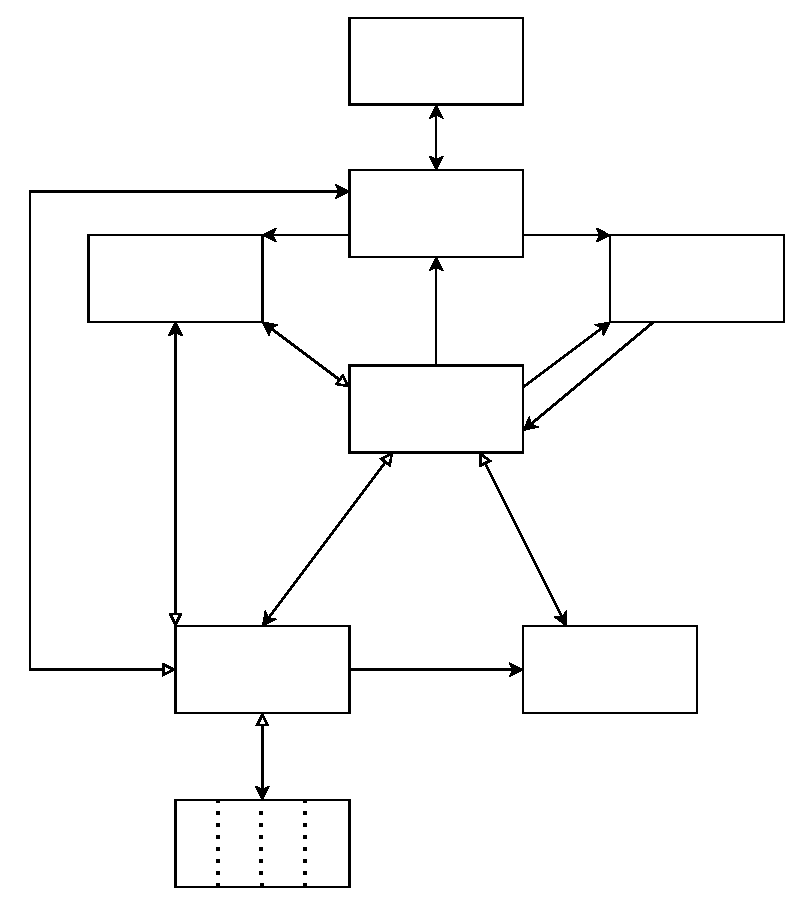
\includegraphics[width=\unitlength]{diagrams/KofferKonzept.eps}}%
    \put(0.36229892,0.75268833){\rotatebox{-37.00000005}{\makebox(0,0)[lt]{\lineheight{1.25}\smash{\begin{tabular}[t]{l}Regel\end{tabular}}}}}%
    \put(0.33445225,0.73951302){\rotatebox{-37.00000005}{\makebox(0,0)[lt]{\lineheight{1.25}\smash{\begin{tabular}[t]{l}anfragen\end{tabular}}}}}%
    \put(0.29118764,0.71969367){\rotatebox{-37.00000005}{\makebox(0,0)[lt]{\lineheight{1.25}\smash{\begin{tabular}[t]{l}Regel senden\end{tabular}}}}}%
    \put(0.66688184,0.62147216){\rotatebox{39.00000116}{\makebox(0,0)[lt]{\lineheight{1.25}\smash{\begin{tabular}[t]{l}Regel auslösen\end{tabular}}}}}%
    \put(0.67293725,0.71663924){\rotatebox{35.99999868}{\makebox(0,0)[lt]{\lineheight{1.25}\smash{\begin{tabular}[t]{l}Job\end{tabular}}}}}%
    \put(0.67209931,0.68230949){\rotatebox{35.99999868}{\makebox(0,0)[lt]{\lineheight{1.25}\smash{\begin{tabular}[t]{l}anlegen\end{tabular}}}}}%
    \put(0.46048854,0.76662729){\makebox(0,0)[lt]{\lineheight{1.25}\smash{\begin{tabular}[t]{l}Daten\end{tabular}}}}%
    \put(0.45394235,0.73934647){\makebox(0,0)[lt]{\lineheight{1.25}\smash{\begin{tabular}[t]{l}senden\end{tabular}}}}%
    \put(0.63499902,0.5214145){\rotatebox{-62.99999795}{\makebox(0,0)[lt]{\lineheight{1.25}\smash{\begin{tabular}[t]{l}Datenantwort\end{tabular}}}}}%
    \put(0.59405085,0.52215864){\rotatebox{-62.99999795}{\makebox(0,0)[lt]{\lineheight{1.25}\smash{\begin{tabular}[t]{l}Datenanfrage\end{tabular}}}}}%
    \put(0.29373901,0.38109393){\rotatebox{52.99999995}{\makebox(0,0)[lt]{\lineheight{1.25}\smash{\begin{tabular}[t]{l}Sensorik anfragen\end{tabular}}}}}%
    \put(0.31158684,0.3594479){\rotatebox{52.99999995}{\makebox(0,0)[lt]{\lineheight{1.25}\smash{\begin{tabular}[t]{l}Aktuatorik auslösen\end{tabular}}}}}%
    \put(0.34596253,0.34802111){\rotatebox{52.99999995}{\makebox(0,0)[lt]{\lineheight{1.25}\smash{\begin{tabular}[t]{l}Ergebnismeldung\end{tabular}}}}}%
    \put(0.44225059,0.29505876){\makebox(0,0)[lt]{\lineheight{1.25}\smash{\begin{tabular}[t]{l}Daten speichern\end{tabular}}}}%
    \put(0.16700054,0.3587181){\rotatebox{90}{\makebox(0,0)[lt]{\lineheight{1.25}\smash{\begin{tabular}[t]{l}Sensor- / Aktuatordefinition\end{tabular}}}}}%
    \put(0.19428137,0.44506678){\rotatebox{90}{\makebox(0,0)[lt]{\lineheight{1.25}\smash{\begin{tabular}[t]{l}anfragen\end{tabular}}}}}%
    \put(0.2390998,0.35871808){\rotatebox{90}{\makebox(0,0)[lt]{\lineheight{1.25}\smash{\begin{tabular}[t]{l}Sensor- / Aktuatordefinition\end{tabular}}}}}%
    \put(0.26638063,0.45106489){\rotatebox{90}{\makebox(0,0)[lt]{\lineheight{1.25}\smash{\begin{tabular}[t]{l}Antwort\end{tabular}}}}}%
    \put(0.34119583,0.97318209){\makebox(0,0)[lt]{\lineheight{1.25}\smash{\begin{tabular}[t]{l}Kommunikation\end{tabular}}}}%
    \put(0.25582146,0.87380195){\makebox(0,0)[lt]{\lineheight{1.25}\smash{\begin{tabular}[t]{l}Konfigurieren\end{tabular}}}}%
    \put(0.66454665,0.86990468){\makebox(0,0)[lt]{\lineheight{1.25}\smash{\begin{tabular}[t]{l}Job anlegen\end{tabular}}}}%
    \put(0.15552789,0.17229505){\makebox(0,0)[lt]{\lineheight{1.25}\smash{\begin{tabular}[t]{l}Ansteuerung\end{tabular}}}}%
    \put(0.32405396,0.17034641){\makebox(0,0)[lt]{\lineheight{1.25}\smash{\begin{tabular}[t]{l}Ergebnis\end{tabular}}}}%
    \put(0.21876703,0.05147997){\makebox(0,0)[lt]{\lineheight{1.25}\smash{\begin{tabular}[t]{l}S1\end{tabular}}}}%
    \put(0.39149484,0.05147997){\makebox(0,0)[lt]{\lineheight{1.25}\smash{\begin{tabular}[t]{l}...\end{tabular}}}}%
    \put(0.03666145,0.29895601){\makebox(0,0)[lt]{\lineheight{1.25}\smash{\begin{tabular}[t]{l}Ansteuerung\end{tabular}}}}%
    \put(0.07268066,0.2658293){\makebox(0,0)[lt]{\lineheight{1.25}\smash{\begin{tabular}[t]{l}Ergebnis\end{tabular}}}}%
    \put(0.32983897,0.05147997){\makebox(0,0)[lt]{\lineheight{1.25}\smash{\begin{tabular}[t]{l}A1\end{tabular}}}}%
    \put(0.70147929,0.28141834){\makebox(0,0)[lt]{\lineheight{1.25}\smash{\begin{tabular}[t]{l}Datenbank\end{tabular}}}}%
    \put(0.26185003,0.30869916){\makebox(0,0)[lt]{\lineheight{1.25}\smash{\begin{tabular}[t]{l}Sensor \&\end{tabular}}}}%
    \put(0.26602133,0.28141834){\makebox(0,0)[lt]{\lineheight{1.25}\smash{\begin{tabular}[t]{l}Aktuator\end{tabular}}}}%
    \put(0.24814873,0.2521889){\makebox(0,0)[lt]{\lineheight{1.25}\smash{\begin{tabular}[t]{l}Schnittstelle\end{tabular}}}}%
    \put(0.49032692,1.08620265){\makebox(0,0)[lt]{\lineheight{1.25}\smash{\begin{tabular}[t]{l}Restliches\end{tabular}}}}%
    \put(0.50402824,1.05697319){\makebox(0,0)[lt]{\lineheight{1.25}\smash{\begin{tabular}[t]{l}System\end{tabular}}}}%
    \put(0.81644849,0.78806221){\makebox(0,0)[lt]{\lineheight{1.25}\smash{\begin{tabular}[t]{l}Scheduler\end{tabular}}}}%
    \put(0.12337549,0.79001084){\makebox(0,0)[lt]{\lineheight{1.25}\smash{\begin{tabular}[t]{l}Definitionen\end{tabular}}}}%
    \put(0.45397279,0.62048002){\makebox(0,0)[lt]{\lineheight{1.25}\smash{\begin{tabular}[t]{l}Regelausführer\end{tabular}}}}%
    \put(0.27235437,0.05147997){\makebox(0,0)[lt]{\lineheight{1.25}\smash{\begin{tabular}[t]{l}S2\end{tabular}}}}%
    \put(0.46310699,0.87575058){\makebox(0,0)[lt]{\lineheight{1.25}\smash{\begin{tabular}[t]{l}Schnittstelle\end{tabular}}}}%
  \end{picture}%
\endgroup%
